\documentclass[../../main.tex]{subfiles}
\begin{document}
\section{Experiments}

To access efficiency of both algorithms, and their MapReduce frameworks set of experiments was performed on the data just described. Two different forms of tests were performed; some for measuring the precision of the algorithms, and some for measuring the speed of the algorithms.\\

As it is only desired to test the speed of {\bf MM} and {\bf MM½} on RNA and DNA, only input of the same form as the \texttt{fasta} file format will be accepted as input.
 
For all experiments, $\epsilon=0.95$. The {\bf MM} clustering algorithm will be referred to as {\bf MM}, likewise will the {\bf MM½} clustering algorithm be referred to as {\bf MM½}. All results from {\tt UCLUST} was retrieved using the {\tt usearch8.0.1517\_win32} version, using the command {\tt cluster\_fast input.fa -id 0.95 -uc clusters.file}. As both {\bf MM} and {\bf MM½} are required to store the clusters, it would be more accurate to demand the same of {\tt UCLUST}, which is what {\tt UCLUST} does onto {\tt clusters.file} using the above command.

\subsection{Precision tests}

In Eq. \ref{minmaxerror}, a metric of the error was set up for the number of hash functions $H$. This error did not provide an answer to relation between $H$ and the size of $k$-mers $k$ and its error. Therefore, a practical testing of this relation was performed, to investigae the precision of {\bf MM} and {\bf MM½}.\\

A gold standard was instrumental to determine the precision of our algorithms. For this purpose, the Levenshtein similarity was used, as defined in Section \ref{sec:levenshtein}. If two strings had a Levenshtein similarity above $\epsilon$ they were placed in the same cluster. The gold standard, \textbf{GS}, were then set to be the number of clusters found by the Levenshtein similarity clustering algorithm. Once the \textbf{GS} were retrieved, the error of an algorithms' found number of clusters, $C$, could be defined as the difference between $C$ and the gold standard \textbf{GS}
$$
E = | C - \mathbf{GS}|
$$

similarly, the percentage of error $E_p$ was 
\begin{equation}\label{eq:errorpercent}
E_p = \frac{|C - \mathbf{GS}|}{\mathbf{GS}}
\end{equation}


The lower $E$ was, the more precise the algorithm. As both {\bf MM} and {\bf MM½} results depend on $k$ and $H$, a large set of tests were performed to determine the precision of each algorithm at many $k$-mer sizes $k$ and number of hash functions $H$. When the optimal settings were found, the results could then be compared to the precision of the \texttt{UCLUST} algorithm. 
\subsubsection{MM precision tests}
First, precision tests of the {\bf MM} algorithm were made. In order to narrow down the number of $k$ and $H$ to test, a heat map of a wide set of $k$ and $H$ for seeing the big scope was made, as seen in Fig. \ref{fig:wideCminmax}. From this wide study, ostensibly the error increased rapidly at $k>13$, and $k<5$ were less precise than $k=5$. Also, at $H>80$ the error seemed to stop changing significantly.

\begin{figure}[H]
\centering
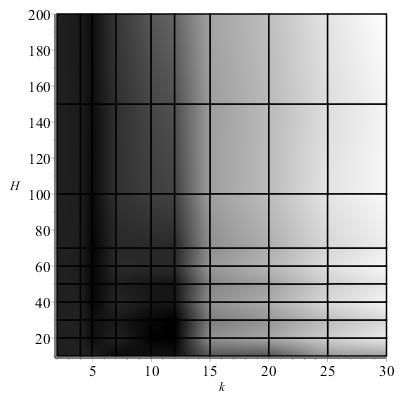
\includegraphics[scale=0.5]{precision/minmax/cecum1wide.jpg}
\caption{Heat map of the error of {\bf MM} at a widely dispersed array of $k$-mer sizes $k$ and number of hash functions $H$, run on \texttt{Cecum1}. Black signifies the smallest error, red the highest error, and yellow medium error relative to black and red.}\label{fig:wideCminmax}
\end{figure}

The results of this test showed that the more rigourous tests could be performed at a more narrow set of $k$ and $H$, as seen in Fig. \ref{fig:Cpreciseminmax}. All heat maps showed very similar results for all samples. There were specific areas that seemed to repeatedly have a very low error, specifically at
\begin{itemize}
\item $k$=5, a black line from $H=50$ to $H=80$.
\item $k=6$, two black spots at around $H=10$ and $H=22$.
\item $k=10,11,12$, two big black spots at around $H=16$ and $H=30$. 
\end{itemize}
These areas of interest were deemed to be most precise. Therefore, each was tested alongside \texttt{UCLUST}, to be able to compare them to each other. Fig. \ref{fig:allKminmax} shows the results of these tests.\\

Fig. \ref{fig:allKminmax}(a) shows that at $k=5$, the overall performance of the algorithm appeared near comparable to \texttt{UCLUST}. At the spikes, the precision was even higher than \texttt{UCLUST}, most notably at $H=54$, $H=65$ and $H=66$, where the average error over all samples can be read from the graph to be approximately 4\%.\\ 

Fig. \ref{fig:allKminmax}(b) shows that at $k=6$, the maximal error is around 70\%, much worse than that of \texttt{UCLUST}. However, two spikes also appeared here at $H=13$ and $H=22$, both with an average error of around 7\%, slightly better than \texttt{UCLUST}.\\

Fig. \ref{fig:allKminmax}(c-e) show that in spite of generally portraying a high error overall at $k=10,11,12$, reaching maximum errors of over 80\%, they still had potentially low errors; Most notably at $k=10,H=20$, $k=11,H=30$, and $k=12,H=30$, with spikes with an average error about 10\%, about the same as \texttt{UCLUST}.\\

\begin{figure}[H]
\begin{subfigure}[b]{.5\textwidth}
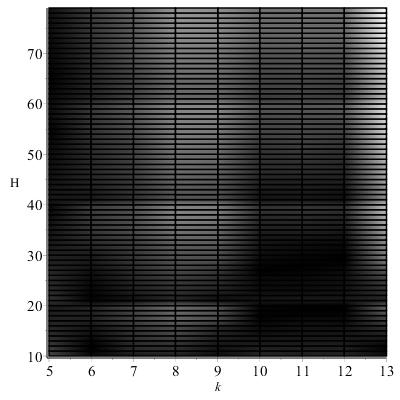
\includegraphics[width=\textwidth]{precision/minmax/cecum1precise}
\caption{\texttt{Cecum1}}
\end{subfigure}
\begin{subfigure}[b]{.5\textwidth}
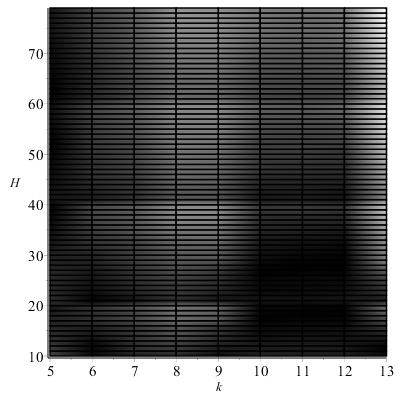
\includegraphics[width=\textwidth]{precision/minmax/cecum2precise}
\caption{\texttt{Cecum2}}
\end{subfigure}
\begin{subfigure}[b]{.5\textwidth}
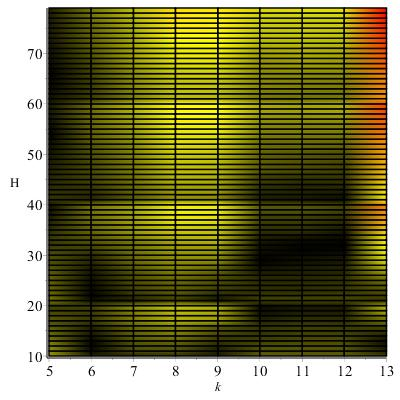
\includegraphics[width=\textwidth]{precision/minmax/cecum3precise}
\caption{\texttt{Cecum3}}
\end{subfigure}
\begin{subfigure}[b]{.5\textwidth}
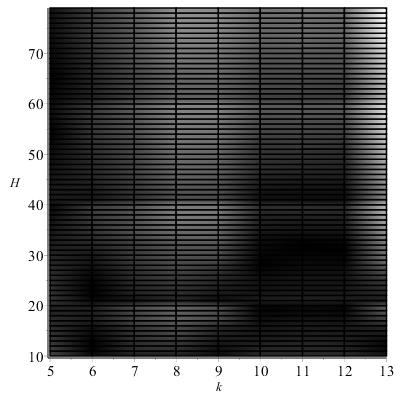
\includegraphics[width=\textwidth]{precision/minmax/cecum4precise}
\caption{\texttt{Cecum4}}
\end{subfigure}
\begin{subfigure}[b]{.5\textwidth}
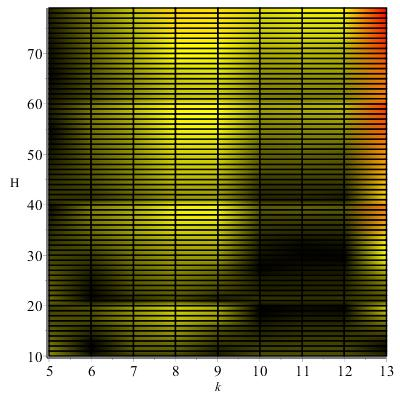
\includegraphics[width=\textwidth]{precision/minmax/cecum5precise}
\caption{\texttt{Cecum5}}
\end{subfigure}
\caption{Heat maps of the error of {\bf MM} at a narrow array of $k$-mer sizes $k$ and numbers of hash functions $H$ at all 5 samples of \texttt{Cecum} DNA. Black signifies the smallest error, red the highest error, and yellow medium error relative to black and red.}\label{fig:Cpreciseminmax}
\end{figure}

\begin{figure}[H]
\begin{subfigure}[b]{.45\textwidth}
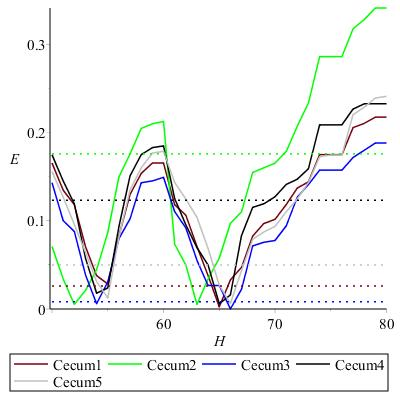
\includegraphics[width=\textwidth]{precision/minmax/k5cecum}
\caption{\texttt{k=5}}
\end{subfigure}
\begin{subfigure}[b]{.45\textwidth}
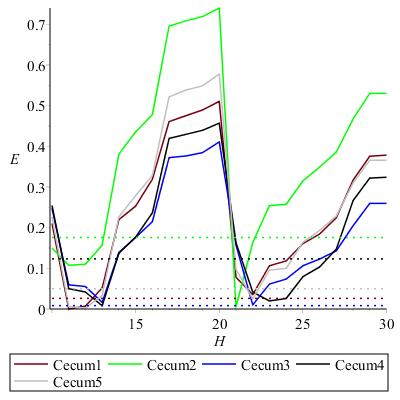
\includegraphics[width=\textwidth]{precision/minmax/k6cecum}
\caption{\texttt{k=6}}
\end{subfigure}
\begin{subfigure}[b]{.45\textwidth}
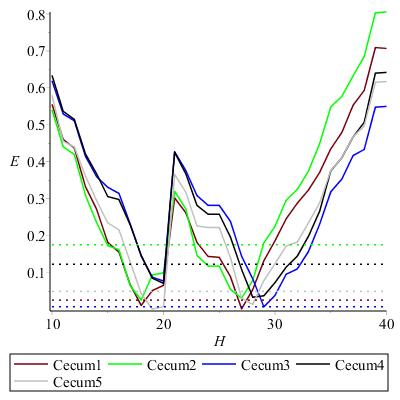
\includegraphics[width=\textwidth]{precision/minmax/k10cecum}
\caption{\texttt{k=10}}
\end{subfigure}
\begin{subfigure}[b]{.45\textwidth}
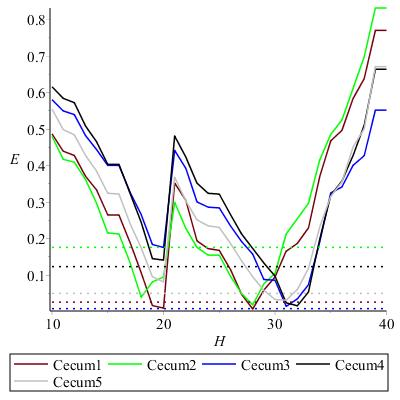
\includegraphics[width=\textwidth]{precision/minmax/k11cecum}
\caption{\texttt{k=11}}
\end{subfigure}
\begin{subfigure}[b]{.45\textwidth}
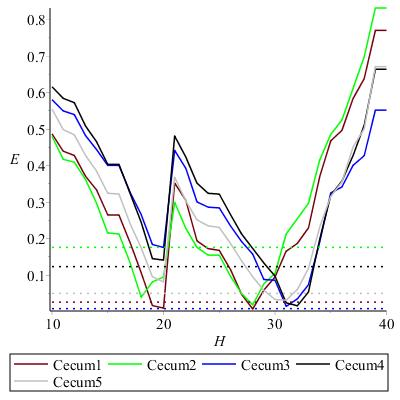
\includegraphics[width=\textwidth]{precision/minmax/k11cecum}
\caption{\texttt{k=10}}
\end{subfigure}
\caption{Plots with hash sizes $H$ on the $x$-axis and error $E_p$ between the test sample and the gold standard in percent $(0.5 = 50\%)$ as defined in Eq. \ref{eq:errorpercent} on the $y$-axis, each plot showing results for a different $k$-mer size $k=5,8,12$. The lines in the plots signify the error at the given $k$ and $H$ of {\bf MM}, while the dotted lines signify the error of \texttt{UCLUST} for each file. Each sample file is given a unique color.}
\label{fig:allKminmax}
\end{figure}

\subsubsection{MM½ precision tests}

The tests of {\bf MM½} were performed completely parallel to those of {\bf MM}, but with lower $H$ as reputedly {\bf MM½} only needs half as many hash functions as the minwise sketch\footnote{see Section \ref{maxmin}}. In Fig. \ref{fig:wiseCminmaxhalf} figures the test of a wide array of $k$ and $H$.
\begin{figure}[H]
\centering
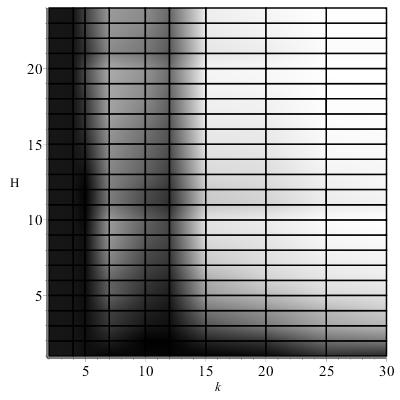
\includegraphics[scale=0.5]{precision/minmaxhalf/cecum1wide.jpg}
\caption{Heat map of the error of {\bf MM½} at a widely dispersed array of $k$ and $H$, run on \texttt{Cecum1}. Black signifies the smallest error, red the highest error, and yellow medium error relative to black and red.}\label{fig:wiseCminmaxhalf}
\end{figure}

The large white plateau in Fig. \ref{fig:wiseCminmaxhalf} meant that $k>15$ could be ignored, as the error at this area was very high. Similarly, $k<5$ gave more error than $k=5$ and could therefore be ignored. $H$ could be reduced to $H< 15$, as the blackest spot seems around $k=5,H=12$.\\

New tests were performed with these limitations. The results can be seen in Fig. \ref{fig:cpreciseminmaxhalf}. All five plot are almost completely identical, showing that mostly at $H=1$ and $H=2$, the precision is highest. The only exception was at $k=5$, where there seemes to be a lower error along all $H$. An additional analysis showed that the minimum error in each heat map of Fig. \ref{fig:cpreciseminmaxhalf} was always at $k=8, H=1$. This result was but a stroke of luck, since a single hash function would theoretically cause the error of the {\bf MM½} sketch to be too high to be applicable for proper comparison (see Eq. \ref{minmaxerror}).\\

For further analysis of the $k$ of interest, the errors of each file at $k=5$, $k=8$, and $k=12$ were plotted, as seen in Fig. \ref{fig:allKminmaxhalf}. Fig. \ref{fig:allKminmaxhalf}(a-c) all have maximum errors that surpass 100\%, even reaching as high as 700\% error. Only in Fig. \ref{fig:allKminmaxhalf}(a) a cuspidate spike was present at $H=12$ with an average error of 20\%, around the double of \texttt{UCLUST} average error.\\


\begin{figure}[H]
\begin{subfigure}[b]{.5\textwidth}
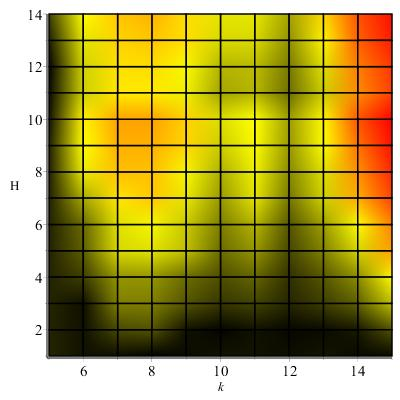
\includegraphics[width=\textwidth]{precision/minmaxhalf/cecum1precise}
\caption{\texttt{Cecum1}}
\end{subfigure}
\begin{subfigure}[b]{.5\textwidth}
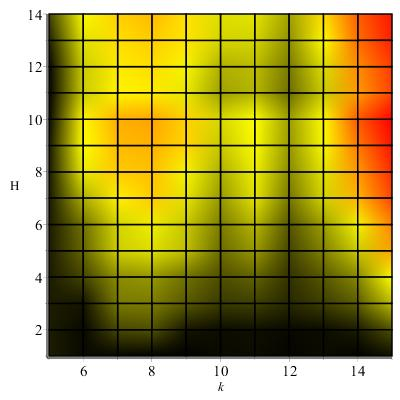
\includegraphics[width=\textwidth]{precision/minmaxhalf/cecum2precise}
\caption{\texttt{Cecum2}}
\end{subfigure}
\begin{subfigure}[b]{.5\textwidth}
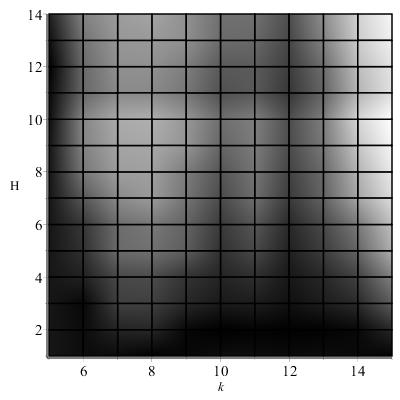
\includegraphics[width=\textwidth]{precision/minmaxhalf/cecum3precise}
\caption{\texttt{Cecum3}}
\end{subfigure}
\begin{subfigure}[b]{.5\textwidth}
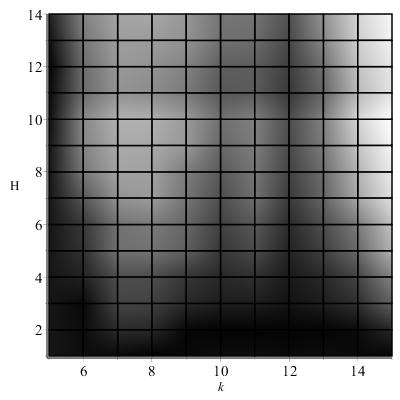
\includegraphics[width=\textwidth]{precision/minmaxhalf/cecum4precise}
\caption{\texttt{Cecum4}}
\end{subfigure}
\begin{subfigure}[b]{.5\textwidth}
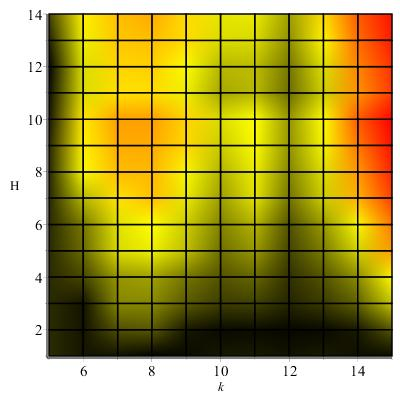
\includegraphics[width=\textwidth]{precision/minmaxhalf/cecum5precise}
\caption{\texttt{Cecum5}}
\end{subfigure}
\caption{Heat maps of the error of {\bf MM½} at a narrow array of $k$ and $H$ at all 5 samples of \texttt{Cecum} DNA. Black signifies the smallest error, red the highest error, and yellow medium error relative to black and red.}
\label{fig:cpreciseminmaxhalf}
\end{figure}

\begin{figure}[H]
\begin{subfigure}[b]{.5\textwidth}
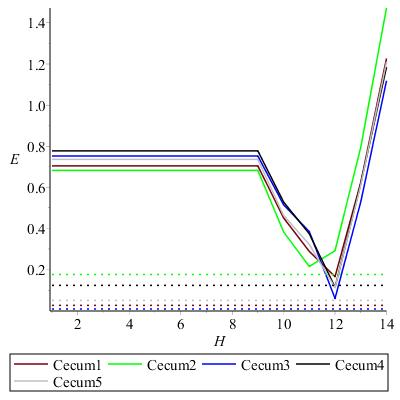
\includegraphics[width=\textwidth]{precision/minmaxhalf/k5cecum}
\caption{\texttt{k=5}}
\end{subfigure}
\begin{subfigure}[b]{.5\textwidth}
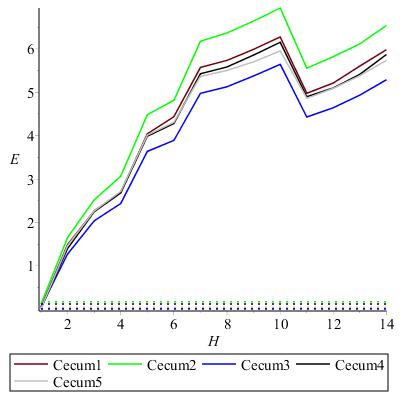
\includegraphics[width=\textwidth]{precision/minmaxhalf/k8cecum}
\caption{\texttt{k=8}}
\end{subfigure}
\begin{subfigure}[b]{.5\textwidth}
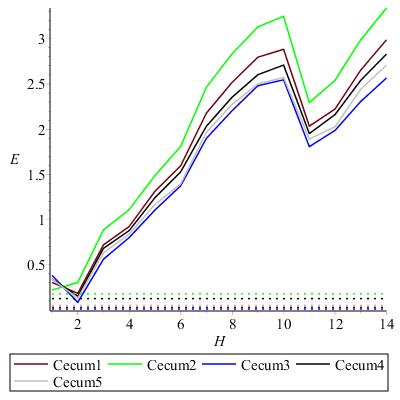
\includegraphics[width=\textwidth]{precision/minmaxhalf/k12cecum}
\caption{\texttt{k=12}}
\end{subfigure}
\caption{Plots with hash sizes $H$ on the $x$-axis and error $E_p$ between the test sample and the gold standard in percent $(0.5 = 50\%)$ as defined in Eq. \ref{eq:errorpercent} on the $y$-axis, each plot showing results for a different $k$-mer size $k=5,8,12$. The lines in the plots signify the error at the given $k$ and $H$ of {\bf MM½}, while the dotted lines signify the error of \texttt{UCLUST} for each file. Each sample file is given a unique color.}
\label{fig:allKminmaxhalf}
\end{figure}

\subsubsection{Comparison}
To determine the precision of {\bf MM}, {\bf MM½} and \texttt{UCLUST}, Fig. \ref{fig:allKminmaxhalf} and Fig. \ref{fig:allKminmax} were perfect candidates. One of the most notable differences between the two graphs was the structure of the results for {\bf MM}, which took an almost "W" like form. The reason for this is from how the sketches of two sequences are compared in Eq. \ref{minmaxjaccard}. In contrast to Eq. \ref{minmaxhalfjaccard}, {\bf MM} takes advantage of the strong points of both the max- and minwise hashing by finding the intersection of jaccards. This means that if the maxwise hashing is most precise at $H=12$, and minwise is most precise at $H=23$, the spikes will appear at these two spots.\\

Comparing the two, {\bf MM} was quite simply much more precise than {\bf MM½}, by very large margin. In fact, at the most precise, {\bf MM½} at $k=5$ was still not as good as the worst {\bf MM} was at $k=5$ in our tests. In fact, {\bf MM} turned out to be even more precise than \texttt{UCLUST} at some very specific parameter settings of $k$ and $H$.\\

The extreme imprecision of {\bf MM½} was in fact so high, that it proved almost nonfunctional for practical purposes, if precision in any way was considered of any importance. {\bf MM} however proved that it could compete with \texttt{UCLUST} in terms of precision. Therefore, {\bf MM} was considered a good candidate for an alternative to \texttt{UCLUST}. What remained was to determine whether it could compare speed-wise.

\subsection{Speed tests}

For testing the speed, the MapReduce Framework using Pig Scripts were taken in use for {\bf MM} and {\bf MM½}. As only the 32 bit version of \texttt{UCLUST} was available, there was a memory limit to the size of the operation. For this reason, some of the sample files could not be finished by \texttt{UCLUST}; this occurence will be noted as Mem. Exed.\\

To achieve the highest speed without loss of too much precision, the precision tests were used to determine the optimal parameters. {\bf MM} was run at $k=6$ and $H=13$, which as seen in Fig. \ref{fig:allKminmax}(b) is comparable to \texttt{UCLUST} in terms of precision. {\bf MM½} was run with $k=5$ and $H=12$. Such low numbers of hash functions were used to increase the speed of the algorithm, and were not by any means the most precise parameters that could be chosen. However, the precision of {\bf MM} at the given $k$ and $H$ was close to the precision of {\tt UCLUST} to be used for the purpose of testing the speed of the algorithm.\\

The results of the test can be seen in Table \ref{tab:speedtest}. As expected, {\bf MM½} was consequently faster than {\bf MM}. Theoretically, {\bf MM½} should be twice as fast as {\bf MM}, which was approximately true in most cases, except for the results of the two samples {\tt Actino500K} and {\tt Actino1mio}. Here {\bf MM½} was respectively 3.5 and 10 times faster than {\bf MM}, caused by the fact that fewer clusters were produced by {\bf MM½}. Therefore the outer loop of the {\bf MM½} greedy algorithm iterated less times than the outer loop of {\bf MM}. Such a difference in speed was not predicted, but says more about the imprecision of {\bf MM½} than the algorithms' relative speed.\\

The reason why {\tt UCLUST} was faster than {\bf MM} in both {\tt Silva50K} and {\tt Actino50K} is because the MapReduce Framework has a long startup time as we noted in Section \ref{sec:mapreduce}. If we had used a single node version of {\bf MM} and {\bf MM½}, we could probably have achieved much higher speeds at samples sizes of 50000 and less, since it would have no startup time. The MapReduce Framework turned out to be advantageous to a single node solution using input files containing more than 50,000 sequences, in the least.\\

Overall, there was a duality of speed between the two sample sets. In the \texttt{Actino} sample set, \texttt{UCLUST} consistently ran faster than both {\bf MM} and {\bf MM½}, with an increasing difference in speed over sample size. In the \texttt{Silva} samples, both {\bf MM} and {\bf MM½} ran faster than \texttt{UCLUST} at sample size higher than {\tt Silva50K}. In fact, {\bf MM} ran\texttt{Silva500K} in 64\% of the time of \texttt{UCLUST}, which completely exceeded the expectations.\\

While the frequency of cases where {\bf MM} and {\bf MM½} are faster than {\tt UCLUST} remains unknown, occasionally {\bf MM} and {\bf MM½} trumps \texttt{UCLUST}. In choosing between {\bf MM½} and {\bf MM}, a strong case could be made for {\bf MM}. {\bf MM½} may have been double as quick as {\bf MM}, but this at the cost of precision. So much precision in fact, that one goes from statistically useless using {\bf MM½} to competing with \texttt{UCLUST} using {\bf MM}. And since {\bf MM} was also quicker than {\tt UCLUST} in some cases, the results suggested that it could serve as an alternative to \texttt{UCLUST}.\\


\begin{table}[H]
\centering
\begin{tabular}{l l l l l l }
\hline
 & \multicolumn{3}{c}{runtime of sample in $s$} & \multicolumn{2}{c}{\% of {\tt UCLUST}}\\
\textbf{Sample} & \textbf{UCLUST} & \textbf{MM} & \textbf{MM½} & \textbf{MM} & \textbf{MM½}\\
\hline \\
\texttt{Actino50K} & 2.0 & 18.3 & 13.6 & 915\% & 680\%\\
\texttt{Actino100K} & 5.0 & 23.2 & 18.7 & 464\% & 374\% \\
\texttt{Actino200K} & 9.0 & 53.4 & 28.8 & 593\% & 320\%\\
\texttt{Actino500K} & 14.0 & 208.4 & 58.3 & 1488\% & 416\% \\
\texttt{Actino1mio} & Mem. Excd. & 1033.8 & 103.3 & & \\
\texttt{Silva50K} & 16.0 & 18.3 & 13.6 & 114\% & 85\% \\
\texttt{Silva100K} & 33.0 & 28.3 & 18.3 & 86\% & 55\%\\
\texttt{Silva200K} & 70.0 & 48.6 & 33.5 & 69\% & 48\% \\
\texttt{Silva500K} & 208.0 & 133.5 & 68.3 & 64\% & 33\%\\
\texttt{Silva1mio} & Mem. Excd. & 273.9 & 128.5 & & \\
\hline
\end{tabular}
\caption{Comparison of clustering speed of three algorithms on 10 samples. \texttt{UCLUST} is run with \texttt{cluster\_fast} option, {\bf MM} with $k$-mer size $k=6$ and $H=13$ number of hash functions, {\bf MM½} with $k$-mer size $k=5$ and $H=12$ number of hash functions. The runtimes of all algorithms are given in seconds. The percentages are the relative speed of {\bf MM} and {\bf MM½} to {\tt UCLUST} in percent.}\label{tab:speedtest}
\end{table}


\end{document}

